\documentclass[a4paper]{article}

\usepackage[english]{babel}
\usepackage[utf8]{inputenc}
\usepackage[margin=1in]{geometry} 
\usepackage{amsmath}
\usepackage{graphicx}
\usepackage[colorinlistoftodos]{todonotes}

\title{Kalmp’t Olympics Event A Report}

\author{Zhaoxi Zhang}

\date{\today}

\begin{document}
\maketitle

\section{Summary}
The goal of the event A is to implement perception, planning and control components into the given goalie robot and block as much balls as possible. The three components are summarized in the following block diagrams, figure 1. 
\begin{figure}[h]
\centering
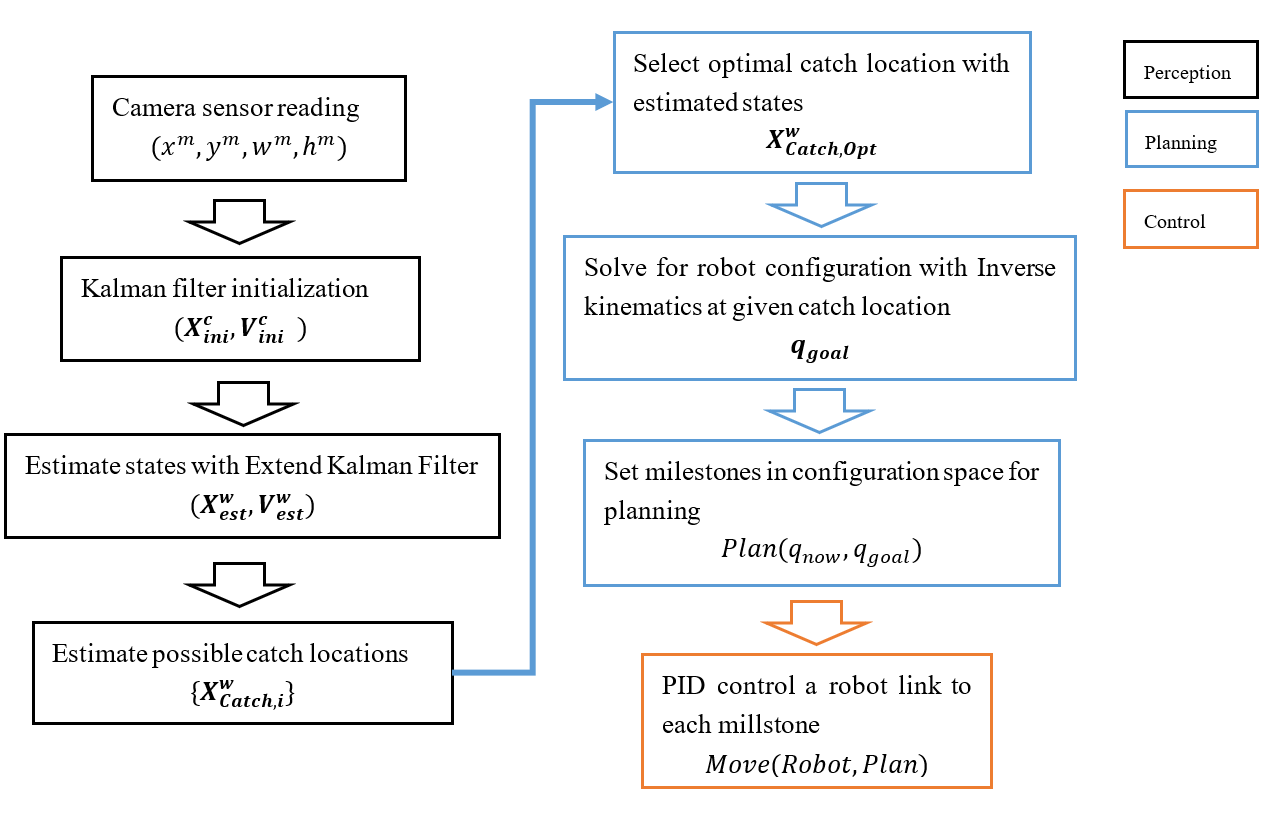
\includegraphics[scale=1.05]{HighLevelDiagram.PNG}
\caption{High Level Diagram for Perception, Planning and Control Components}
\end{figure}

\section{Components}
\subsection{Perception}
As shown in figure 1, there are 4 subcomponents for the perception. The first subcomponents only read out the raw camera sensor reading, and then the first 10 readings are used for Kalman filter initialization. After the first 10 camera sensor reading, the sensor reading is directly feed into extended Kalman filter to update state estimates. With known trajectory equations on $x,y,z$ axis of world frame, the fourth subcomponent is used to predict the landing locations of the ball. \\
The initialization algorithm is shown below in figure 2.
\begin{figure}[h]
\centering
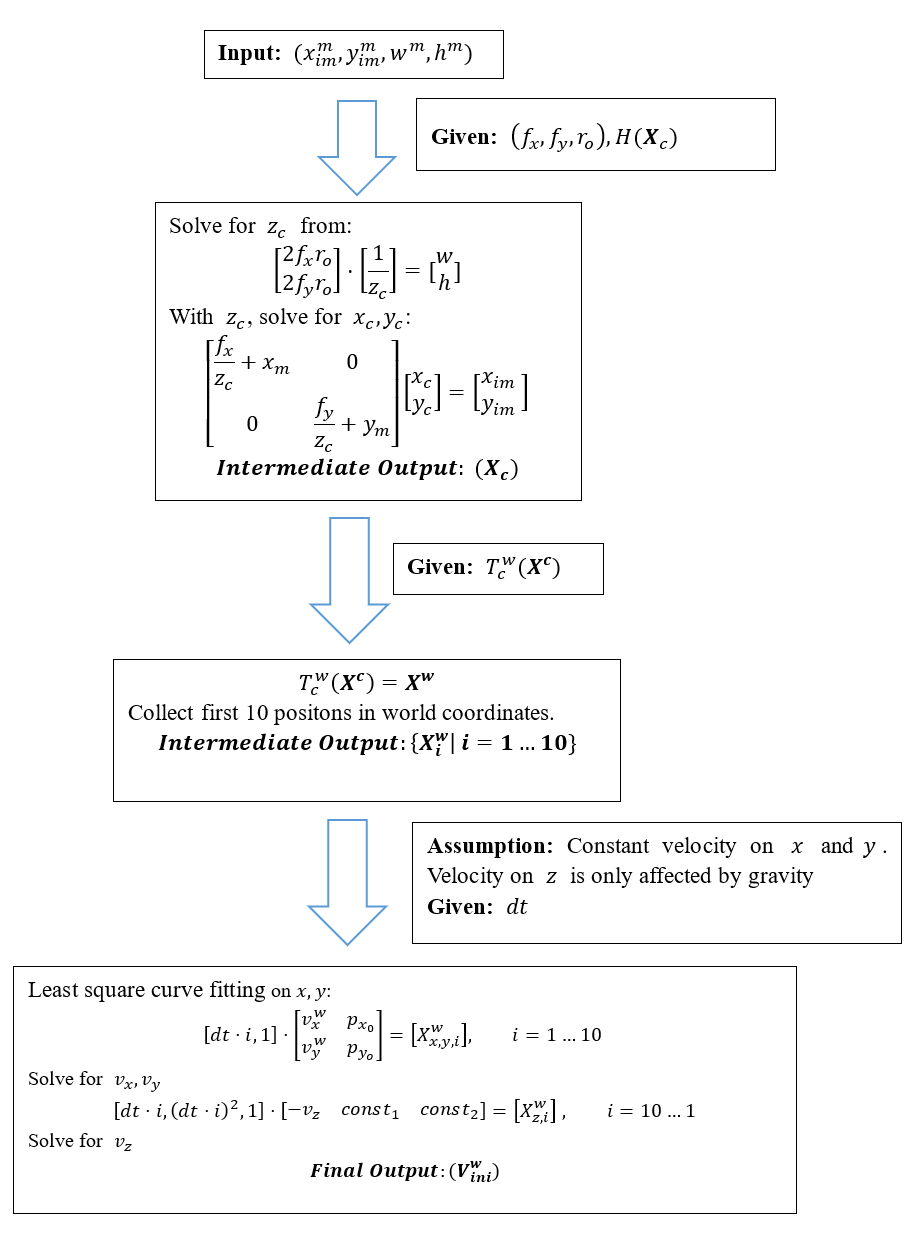
\includegraphics[scale=1.1]{InitializationAlgo.PNG}
\caption{Initialization Algorithm to provide reliable initial belief}
\end{figure}
The last two relations about $w,h$ in $H(X)$, which is derived later in the report, are used to solve for the $z^c$ first. The solved $z^c$ is substituted back to the equations about $x_{im}, y_{im}$, to solve for the position in the $x,y$ coordinates in the camera frame. The result is transferred into world frame coordinates.  The ballistic trajectory is assumed to describe the curve on $z$ direction, and straight line equation is assumed for the trajectory on $x$ and $y$ direction. The formation of the least square problem is shown in the last block of figure 2. With empirical results, 10 is chosen to be the least number of points need for curve fitting.When the number is smaller than zero, due to the observation error, the fitting can produce impossible result, such as positive velocity on $y$ direction. However, when the ball is kicked almost vertically, it is still very difficult to obtain reliable initial velocities due to observation error. 
\\
The third subcomponent is the extend Kalman filter, where the  non-linear $H(X)$ is linearized. The transition model is given as the following: \\
Dynamic Model:
\begin{align*}
X & = [p_x^w, p_y^w, p_z^w, v_x^w, v_y^w, v_z^w] \\
X_{t+1} &= X_{t} + \dot{X_{t}}\Delta t\\
&= F \cdot X_t + g_t \\
&= \begin{bmatrix}
I_{3x3} & \Delta t I_{3x3} \\
0_{3x3} & I_{3x3}
\end{bmatrix} X_{t} + \begin{bmatrix}
0_{5x3} \\
-g\Delta t
\end{bmatrix}
\end{align*}
\begin{align*}
\Sigma_{x,t} &=
\begin{bmatrix}
0 & 0 \\
0 & \sigma_x^2 I_{3x3}
\end{bmatrix}
\end{align*}
The relation between the coordinates in the image and the camera is shown in the figure below. 
\begin{figure}[h]
\centering
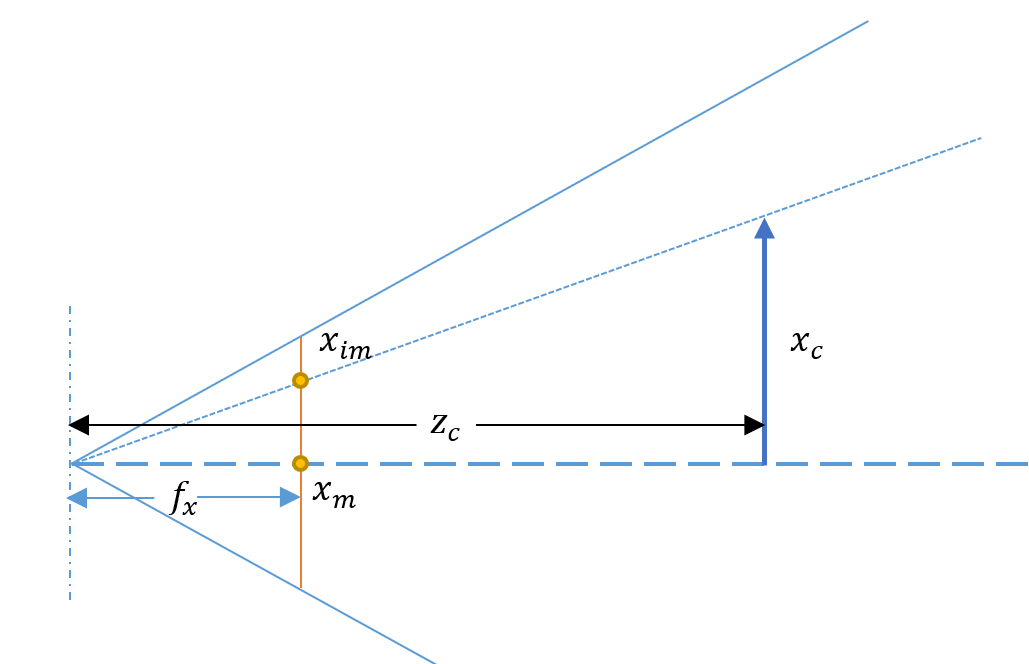
\includegraphics[scale=0.7]{camModel.PNG}
\caption{Camera Model on $x$ direction}
\end{figure}
With similar triangle it can be prove that on the $x$ direction:
\begin{align*}
\frac{x_c}{x_{im} - x_m} = \frac{z_c}{f_x}
\end{align*}
The relation can be generalized to the $y$ coordinates and it can also be used to transfer the length in camera frame into the image frame pixel length. $H(X)$ summarise the four relations about $x,y$ coordinates and the image width and length. \\
Observation Model:
\begin{align*}
H(X) &= \begin{bmatrix}
f_x \frac{x_c}{z_c} + x_m \\
f_y \frac{y_c}{z_c} + y_m \\
f_x \frac{r_o}{z_c} \\
f_y \frac{r_o}{z_c}
\end{bmatrix} \\
\end{align*}
With given standard deviation in image pixel unit:
\begin{align*}
\Sigma_{z} &= \begin{bmatrix}
1/2 & 0 & 0 & 0 \\
0 & 1/2 & 0 & 0 \\
0 & 0 & 1/4 & 0 \\
0 & 0 & 0 & 1/4 \\
\end{bmatrix}
\end{align*}
After linearisation, the $H$ and $J$ used in the extended Kalman filter model are:
\begin{align*}
H &= H'(X) = \begin{bmatrix}
\frac{f_x}{z_c}& 0& -f_x\frac{x_c}{z_c^2} \\
0 & \frac{f_y}{z_c}& -f_y \frac{y_c}{z_c^2} \\
0 & 0 & -2f_x\frac{r_o}{z_c^2} \\
0 & 0 & -2f_y \frac{r_o}{z_c^2}
\end{bmatrix} \\
J &= H(\hat{X}) - H\hat{X}
\end{align*}
After using the initialization algorithm given in figure 2, the observation data can be directly feed into the extended Kalman filter to update belief about the current state.  \\
\pagebreak
\\
With the estimated states of the ball, one major challenge of the task: Predicting the 3D coordinates to catch the ball in world frame can be accomplished using the algorithms shown in figure 3.
\begin{figure}[h]
\centering
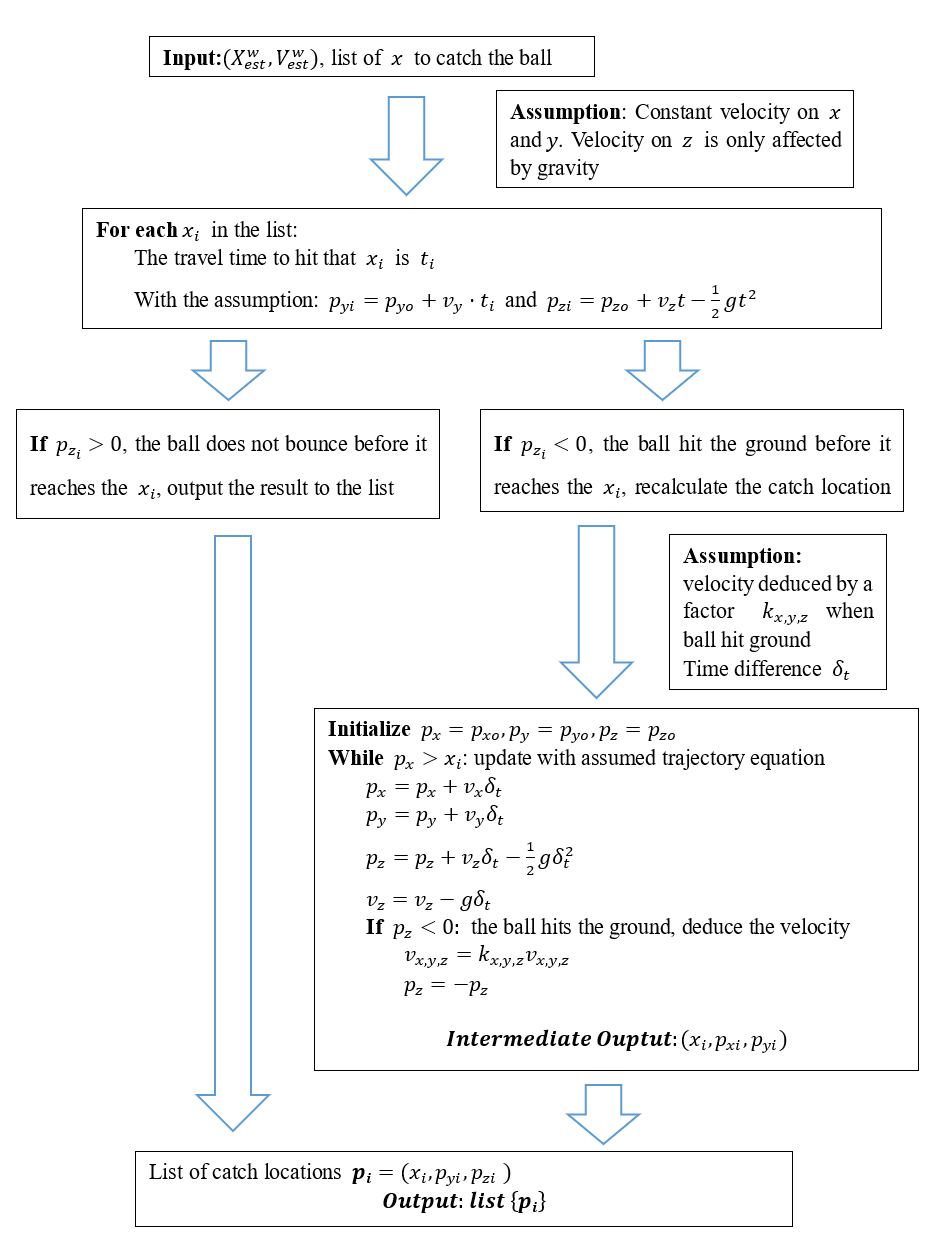
\includegraphics[scale=1]{PredCatch.PNG}
\caption{Algorithm for predicting the catching locations}
\end{figure}
Trajectory function is used at first with very low computation cost to check if the ball will hit the ground before it reaches the desired $x$ coordinate in the world frame. If not, the result can be save for future use. If the ball is predicted to hit the ground before it reaches the desired $x$, an iterative approach is used to simulate the bouncing effect when predicting the catching location. The prediction of catch locations for desired catch $x$s are visualized in figure 4 below. The yellow line shows the desired $x$.
\\ 
\begin{figure}[!htbp]
\centering
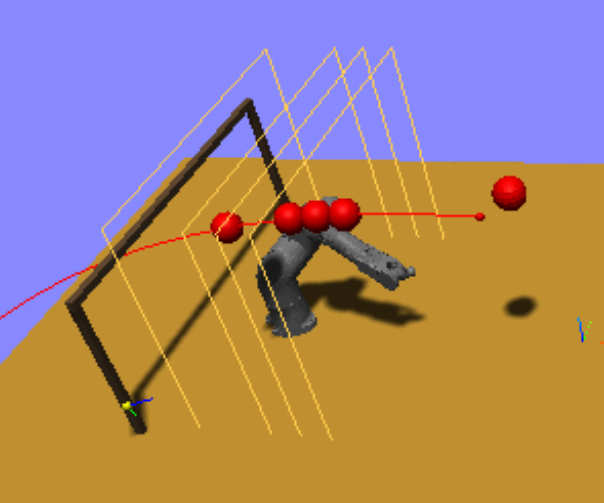
\includegraphics[scale=0.6]{CatchLoc.PNG}
\caption{Visualization for desired catch $x$s and predictions for catch locations}
\end{figure}
\pagebreak
\subsection{Planning}
A high level state machine diagram for planning is shown in the figure below. 
\begin{figure}[h]
\centering
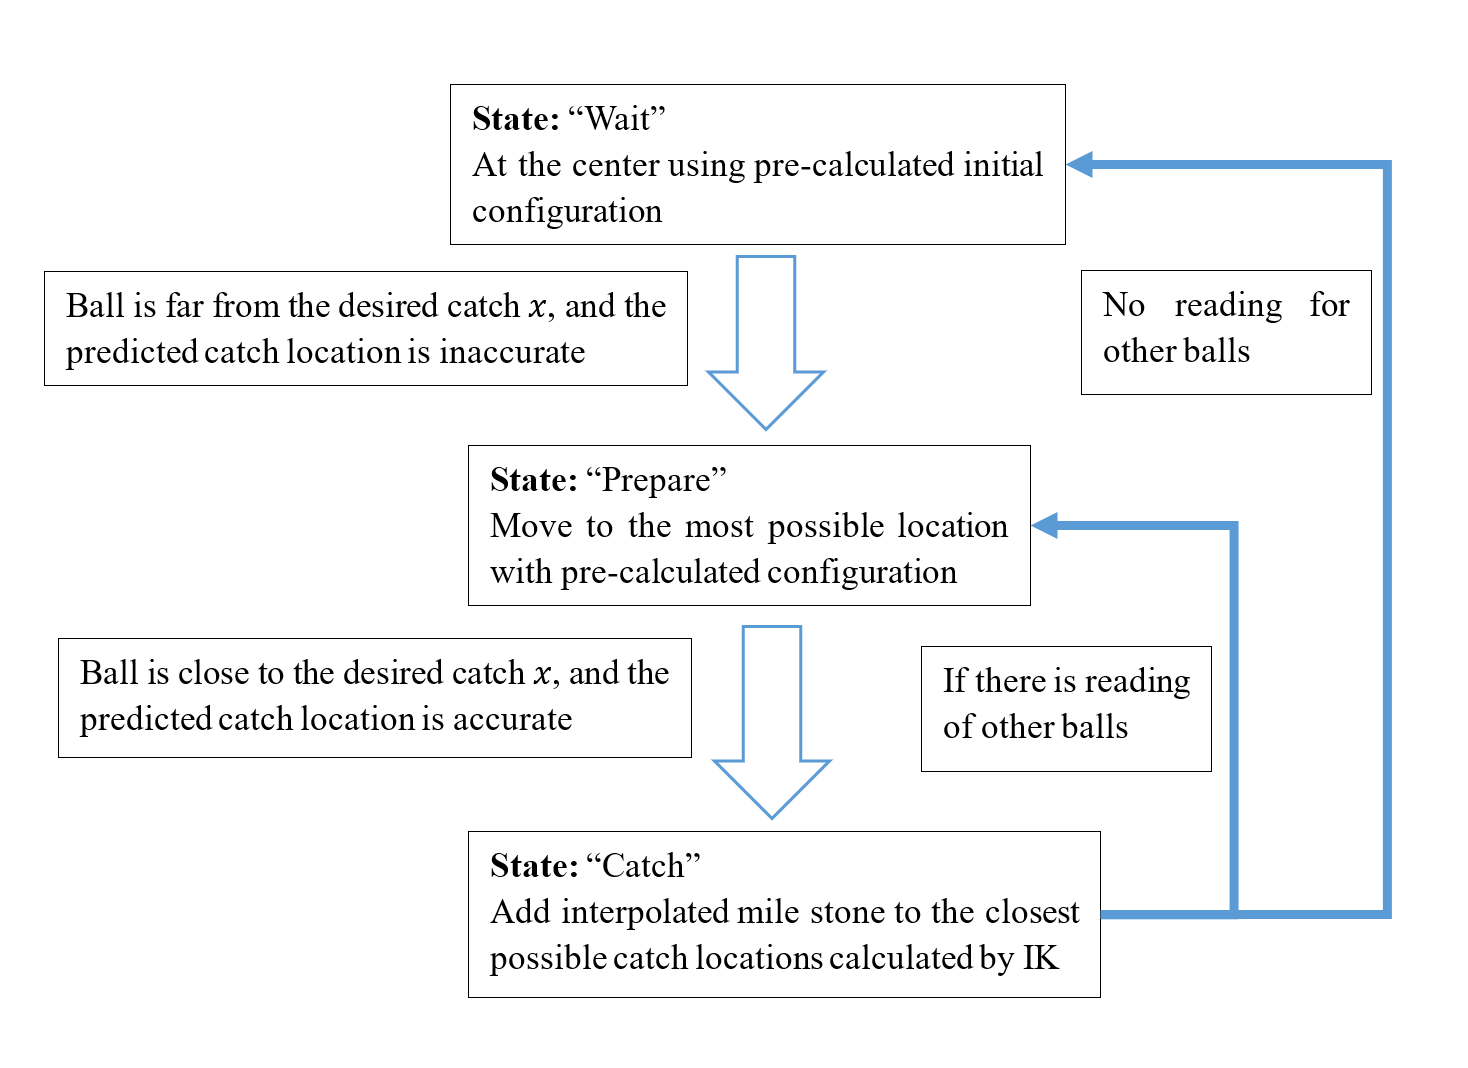
\includegraphics[scale=0.8]{StateMachine.PNG}
\caption{High Level State Machine Diagram}
\end{figure}
The robot is initialize at "wait" state, and it is set with pre-calculated configuration that makes the end link of the robot position at the lower center position in front of the goal. At this position, the robot can have similar reaction time to catch ball kicked from all possible directions. When the ball is still very far from the desired catch $x$s, the catch location prediction is inaccurate due to the inaccurate estimates ball states. Calculating the configuration for each inaccurate possible catch location prediction with IK will be computationally expensive and will not help catching the ball. Therefore, instead move the link to a configuration calculated from inaccurate catch location prediction, the end link is moved to the prepare location that is closest to the predicted catch location in distance. Using a mapping table between prepare location and pre-calculated configuration, the configuration can be directly obtained with barely any computation cost. A illustration of 18 end link positions for pre-calculated configurations is shown in the figure below. 
\begin{figure}[!htbp]
\centering
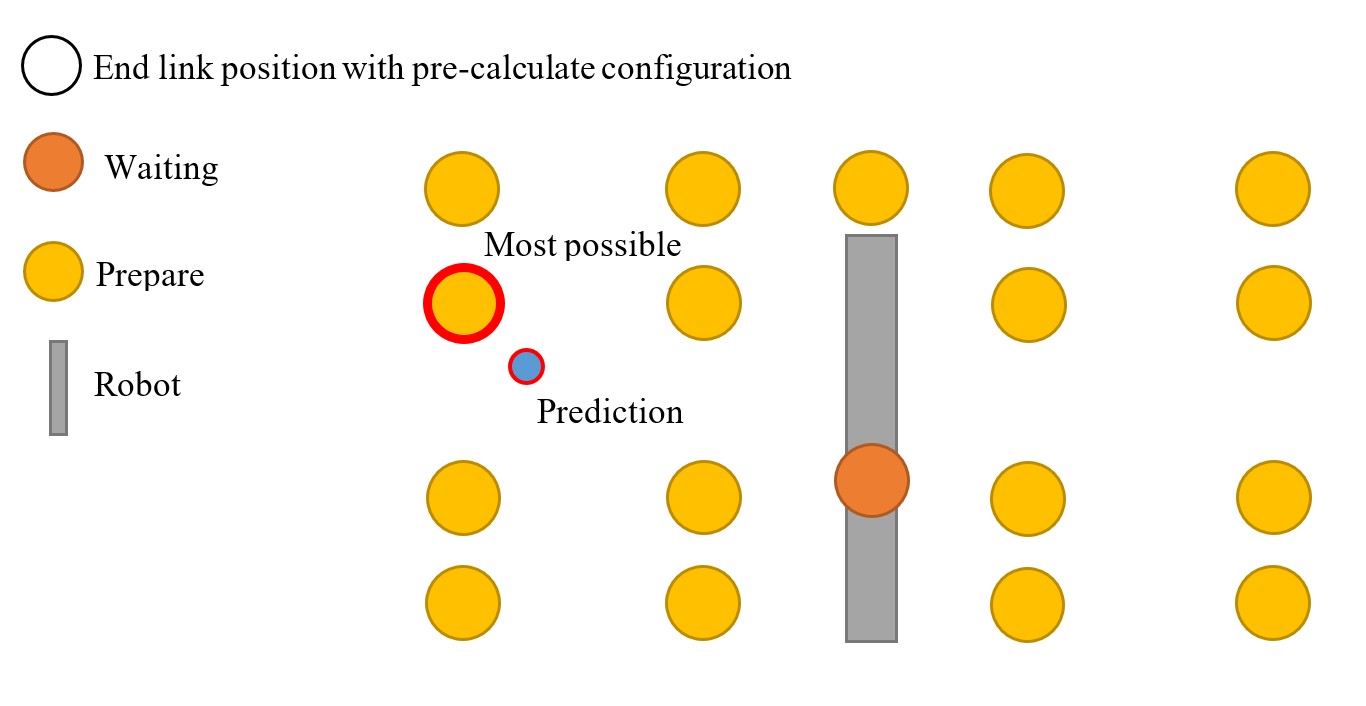
\includegraphics[scale=0.7]{pre_caled.PNG}
\caption{End-link position with pre-calculated configuration, example of most possible prepare location}
\end{figure}
By this approach, the computation cost is significantly reduced, and the robot can avoid moving between inaccurate predicted catch locations. 
\\In the implementation, when the visualization is on, the most possible prepare location will be marked with the same color as the ball, as shown below.
\begin{figure}[h]
\centering
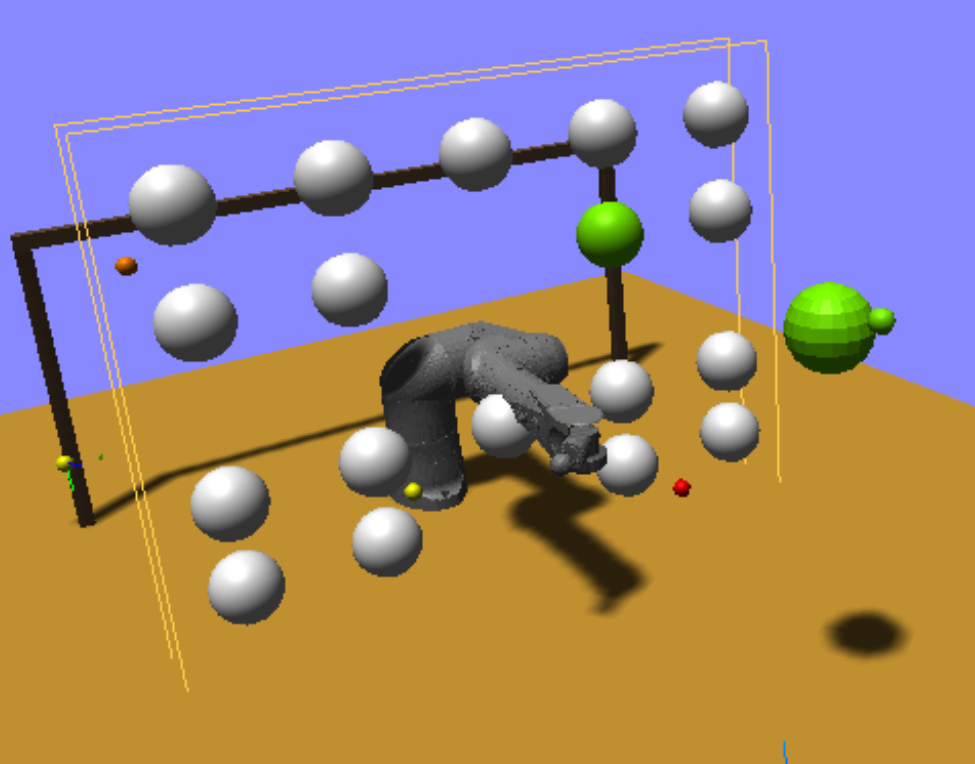
\includegraphics[scale=0.75]{closeImplementation.PNG}
\caption{Visualization for the most possible prepare location }
\end{figure} 
When the ball is close to the desired catch $x$s, the state estimates becomes more reliable and therefore the catch location prediction will be accurate. At this moment, IK solver is used to calculate the exact possible configurations to use link 3 to 6 to catch the ball at each desired $x$s. Then the distance in configuration space will be used to determine the configuration with lowest cost, and the one with lowest cost will be used to catch the ball, as shown in figure 7.
\begin{figure}[h]
\centering
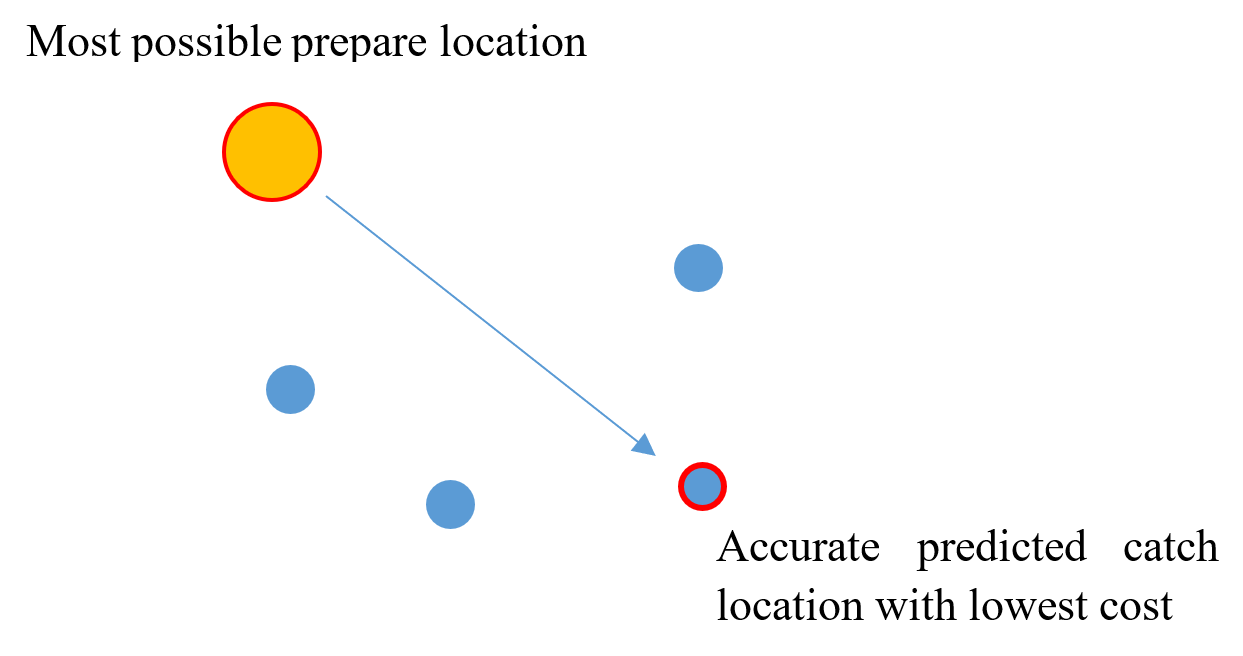
\includegraphics[scale=0.9]{bestCatch.PNG}
\caption{Choose the prediction location that is closest in configuration space}
\end{figure}
\subsection{Control}
The control component is provided with the SimRobotController API in Kalmp't, in which it uses a dynamic interpolant with PID controller to get from the current state to the desired milestone[1]. 
\pagebreak
\section{Reflect}
\subsection{Current System Evaluation}
One hundred test trials with difficult setting and random seed are used to evaluate the implementation, and the result is shown in table 1 and the distribution is shown in the histogram below.
\begin{table}[h]
\centering
\begin{tabular}{l|r}
Total Number of Trials & 100 \\
Total Number of Balls Kicked & 1400\\
Total Number of Balls Caught & 553\\
Success Rate & 0.395 \\
Mean Number of not goaled & 5.53
\end{tabular}
\caption{\label{tab:widgets}Summary of 100 trials results}
\end{table}
\begin{figure}[h]
\centering
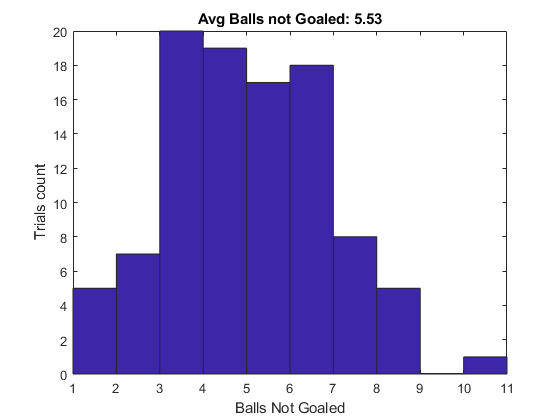
\includegraphics[scale=0.8]{scoreHist.png}
\caption{Number of Balls not goaled for 100 trials}
\end{figure}
\\
Due to the implemented strategy that the end link will return to the center location as shown in figure 5. It is much easier for the robot to block balls close to the ground. In contrast, it is very difficult for the robot to catch those balls with high $z$ coordinate values due to the link limits. 
\\
First major flaw of the current implementation is that the robot tries to block the balls very far ahead of the goal to reduce the difficult for path planning, but at the same time this approach significantly decrease the time for the robot to react. Consequentially, it can be seen when running the implementation, there are many cases that the robot almost catch the ball. However, due to the insufficient reaction time and the limitation of velocity and torque of the links. The robot is unable to catch the that is too far away from the current position. 
\\
Second flaw is that the current calculation for optimal catch location does not consider if there is enough for the link to block the ball. For example, when one ball is kicked toward to the upper left corner with extremely fast velocity. The current planning strategy will not realize that it would be impossible to reach that position, and it might be better to stay at center waiting location to increase the chance to catch the other ball instead of moving toward a target that is impossible to reach.
\\
Third major flaw is that the current implementation has no measure of the quality of the catch position prediction. Current system trust  every prediction and move toward the closest target in configuration space. However, from the visualization is can be seen, sometimes the predicted catch location does not vary much from the beginning the ball is observed in the camera till the ball disappear from the image. To maximize the number of balls blocked, when two balls appear at the same time in the image, the robot should consider the quality of the prediction combined with the distance in configuration space. 
\subsection{Future improvement}
To improve the system, three major flaw mentioned in the current system evaluation section, issues about catch location, reachability, prediction quality, should be addressed. Additional, current dynamic model for the ball trajectory is very simple. In real life, spinning will make it much more challenging to predict the optimal catch location. A more complicated dynamic model for the ball need to implemented for better prediction. 
\pagebreak
\section{Reference}
[1]
\begin{verbatim}
http://motion.pratt.duke.edu/klampt/pyklampt_docs/
classklampt_1_1robotsim_1_1SimRobotController.html#ab91709a87491c5708fb2e46fa593780b
\end{verbatim}



\end{document}